\documentclass[a4paper,11pt,oneside]{article}

% To use this template, you have to have a halfway complete LaTeX
% installation and you have to run pdflatex, followed by bibtex,
% following by one-two more pdflatex runs.
%
% Note thad usimg a spel chequer (e.g. ispell, aspell) is generolz
% a very guud ideo.

\usepackage[a4paper,top=3cm,bottom=3cm,left=3cm,right=3cm]{geometry}
\renewcommand{\familydefault}{\sfdefault}

\usepackage{helvet}
\usepackage{wrapfig}
\usepackage{color}

\usepackage{parskip}		%% blank lines between paragraphs, no indent
\usepackage[pdftex]{graphicx}	%% include graphics, preferrably pdf
\usepackage[pdftex]{hyperref}	%% many PDF options can be set here
\pdfadjustspacing=1		%% force LaTeX-like character spacing
\usepackage[bottom]{footmisc}	%% sends footnotes to bottom of page
\usepackage{float}		%% figure placement 

\newcommand{\myname}{Samirah Amadu - 11809737 \& Inti Gabriel Mendoza Estrada - 11804156}
\newcommand{\mytitle}{Linear Classification}
\newcommand{\mysupervisor}{Assoc. Prof. Dipl.-Ing. Dr. techn. Robert Legenstein}

\renewcommand{\labelenumii}{\theenumii}
\renewcommand{\theenumii}{\theenumi.\arabic{enumii}.}

\usepackage{xcolor,listings}
\usepackage{textcomp}
\usepackage{color}
\usepackage{hyperref}

\definecolor{codegreen}{rgb}{0,0.6,0}
\definecolor{codegray}{rgb}{0.5,0.5,0.5}
\definecolor{codepurple}{HTML}{C42043}
\definecolor{backcolour}{HTML}{F2F2F2}
\definecolor{bookColor}{cmyk}{0,0,0,0.90} 
\definecolor{codegreen}{rgb}{0.13,0.54,0.13}
\color{bookColor}

\lstset{upquote=true}

\lstdefinestyle{mystyle}{
    backgroundcolor=\color{backcolour},   
    commentstyle=\color{codegray},
    keywordstyle=\color{codepurple},
    numberstyle=\numberstyle,
    stringstyle=\color{codegreen},
    basicstyle=\footnotesize\ttfamily,
    breakatwhitespace=false,
    breaklines=true,
    captionpos=b,
    keepspaces=true,
    numbers=left,
    numbersep=10pt,
    showspaces=false,
    showstringspaces=false,
    showtabs=false,
}
\lstset{style=mystyle}

\newcommand\numberstyle[1]{%
    \footnotesize
    \color{codegray}%
    \ttfamily
    \ifnum#1<10 0\fi#1 |%
}



\hypersetup{
  pdfauthor = {\myname},
  pdftitle = {\mytitle},
  pdfkeywords = {},
  colorlinks = {true},
  linkcolor = {blue},
  citecolor = {blue},
  urlcolor = {blue}
}

\begin{document}
  \pagenumbering{roman}

  \thispagestyle{empty}

  \begin{flushright}
    
\includegraphics[scale=0.25]{TU_Graz.png}
  \end{flushright}
  \vspace{20mm}
  \begin{center}
    \huge
    \textbf{\mytitle}
  \end{center}
  \vspace*{4mm}
  \begin{center}
   \Large by
  \end{center}
  \vspace*{4mm}
  \begin{center}
    \Large
    \textbf{\myname}
  \end{center}
  \vspace*{20mm}
  \begin{center}
    \large
    Neural Networks KU WS19 - Exercise Sheet 2
  \end{center}
  \vfill
  \begin{flushright}
    \large
    \begin{tabular}{c}
      \mysupervisor \\
      \hline
      Name and title of the supervisor \\
      \\
    \end{tabular}
  \end{flushright}
  \vspace*{8mm}
  \begin{flushleft}
    \large
    Date of Submission: \today \\
    \rule{\textwidth}{1pt}
  \end{flushleft}
  \begin{center}
    \Large TU Graz --- Computer Science Masters Programme
  \end{center}

  \newpage
  \tableofcontents

  \clearpage
  \pagenumbering{arabic}

\section{Introduction}
  Given a dataset \texttt{vehicle.pkl}, we aim to classify a given silhouette as one of two types of vehicles, i.e., \texttt{SAAB} or \texttt{VAN}. To do so, we use a \textit{Probabilistic Generative Model} approach that allows us to classify our dataset as well as the \texttt{Iterative Reweighted Least Squares (IRLS)} algorithm. We will compare and contrast each model's performance on our \texttt{vehicle.pkl} dataset.

The dataset consists of 270 training examples and 146 test examples which each have 18 features characterizing the object. There are two classes (\texttt{vehicle.pkl} has 4 `classes' but we only extract 2 of them) of interest: SAAB (Class tag 2) and VAN (Class tag 4).

We aim to minimize misclassification rate on the test set after training with either algorithm. The entire code can be found in the \texttt{nn19\_task2.py} file.

\newpage

\section{Implementation}

We used Python 3.7.0 to develop our implementation of the algorithms. To extract the dataset from \texttt{vehicle.pkl} we use:
\begin{lstlisting}[ language=Python,
                    deletekeywords={IDENTITY},
                    deletekeywords={[2]INT},
                    morekeywords={clustered, AUTO_INCREMENT, np},
                    framesep=8pt,
                    xleftmargin=40pt,
                    framexleftmargin=40pt,
                    frame=tb,
                    framerule=0pt ]
# Training set
X = vehicle_data['train']['X']  # features; X[i,j]...feature j of example i
C = vehicle_data['train']['C']  # classes; C[i]...class of example i
# Test set
Xtst = vehicle_data['test']['X']  # features
Ctst = vehicle_data['test']['C']  # classes

# extract examples of class SAAB (2) and VAN (4)
indices = np.flatnonzero((C == 4) | (C == 2))
C = C[indices]
X = X[indices]

indices_tst = np.flatnonzero((Ctst == 4) | (Ctst == 2))
Ctst = Ctst[indices_tst]
Xtst = Xtst[indices_tst]
\end{lstlisting}

\subsection{Probabilistic Generative Model}

We use the \textit{Probabilistic Generative Model} approach to classify the data set, assuming Gaussian class-conditional distributions with a common covariance matrix. To estimate the class prior probability, covariance matrix, the means, and the posterior distribution, from the training data, we do:
	\begin{lstlisting}[ language=Python,
                    deletekeywords={IDENTITY},
                    deletekeywords={[2]INT},
                    morekeywords={clustered, AUTO_INCREMENT, np},
                    framesep=8pt,
                    xleftmargin=40pt,
                    framexleftmargin=40pt,
                    frame=tb,
                    framerule=0pt ]
# find prior probability
nr_training_examples = C.size

unique, examples_per_class = np.unique(C, return_counts=True)  # counts .. number of examples per class, unique .. classes
prior = examples_per_class / nr_training_examples  # convert count into percentage
priors = dict(zip(unique, prior))

# find mean for each class
mean = {}
i = 0
for cls in unique:
    mean[cls] = (1/examples_per_class[i]) * np.sum(X[np.flatnonzero(C == cls)], axis=0)
    mean[cls] = mean[cls].reshape((-1, 1))
    i = i+1

# compute covariance matrix
s = {}
normalized_features = {}
for cls in unique:
    indices = np.flatnonzero(C == cls)
    normalized_features[cls] = X[indices].T - mean[cls]

j = 0
for cls in unique:
    s[cls] = (1/examples_per_class[j]) * (normalized_features[cls] @ normalized_features[cls].T)
    j = j+1

covariance = (examples_per_class[0]/nr_training_examples) * s[unique[0]] + \
             (examples_per_class[1]/nr_training_examples) * s[unique[1]]

# compute posterior probability
sigmoid = lambda a: np.where(a >= 0, 1 / (1 + np.exp(-a)), np.exp(a) / (1 + np.exp(a))) # numerically stable
\end{lstlisting}

From the lecture notes we get the \textit{Gaussian-Class Conditionals With Common Covariance Matrix}:

If $p(\textbf{x}|C_k) \sim \mathcal{N}(\mu_k, \Sigma)$, then we arrive at:
\begin{eqnarray*}
p(C_1|x)	&	=	&	\sigma(\textbf{w}^T\textbf{x} + w_0) \textrm{ with}\\
\textbf{w}	&	=	&	\Sigma^{-1}(\mu_1 - \mu_2)\textrm{,}\\
w_0	&	=	&	-\frac{1}{2}\mu_1^T\Sigma^{-1}\mu_1 + \frac{1}{2}\mu_2^T\Sigma^{-1}\mu_2 + ln\frac{p(C_1)}{p(C_2)}\textrm{.}
\end{eqnarray*}
We implement this in Python as:
\begin{lstlisting}[ language=Python,
                    deletekeywords={IDENTITY},
                    deletekeywords={[2]INT},
                    morekeywords={clustered, AUTO_INCREMENT, function, document, var, np},
                    framesep=8pt,
                    xleftmargin=40pt,
                    framexleftmargin=40pt,
                    frame=tb,
                    framerule=0pt ]
def classify(X, mean, covariance, target, flag="train"):
    result = np.zeros((X.shape[1]-1, 2), dtype=float)
    for features in range(2, X.shape[1]+1):
        sub_m1 = mean[2][0:features]
        sub_m2 = mean[4][0:features]
        covinverse = np.linalg.pinv(covariance[0:features, 0:features]) # Simga^-1
        weights = covinverse @ (sub_m1 - sub_m2) # w
        bias = (-(1/2) * sub_m1.reshape((1, -1)) @ covinverse @ sub_m1) \
               + ((1/2) * sub_m2.reshape((1, -1)) @ covinverse @ sub_m2) \
               + np.log(priors[2]/priors[4]) # w_0
        input = X[:, 0:features]
        prediction = (sigmoid(weights[0:features].reshape((1, -1)) @ input.T + bias)) # p(C_1|x)
        [...] # out of scope code

    return result
\end{lstlisting}

If our \texttt{prediction} variable (seen above) is smaller than 0.5, the object is classified as \texttt{VAN}, else as \texttt{SAAB}. We are able to do the classification using only the first 2, then 3, etc\dots up to all features of the dataset through the \texttt{for} loop. The dataset is a table in which the columns are the features, therefore using \texttt{[0:features]} allows us to partition the array/table by the specified amount of features for each iteration. 

We are able, then, to plot the classification accuracy (percentage of correctly classified examples) as a function of the number of input features for both the training set and the test set. 

The training correct classification percentage on the training set reaches a 98.52\% and 94.52\% on the test set `at' 18 features. Note that the misclassification rate is just (1.0 - \texttt{Accuracy}). The full graph can be seen below:

\hspace*{-2cm}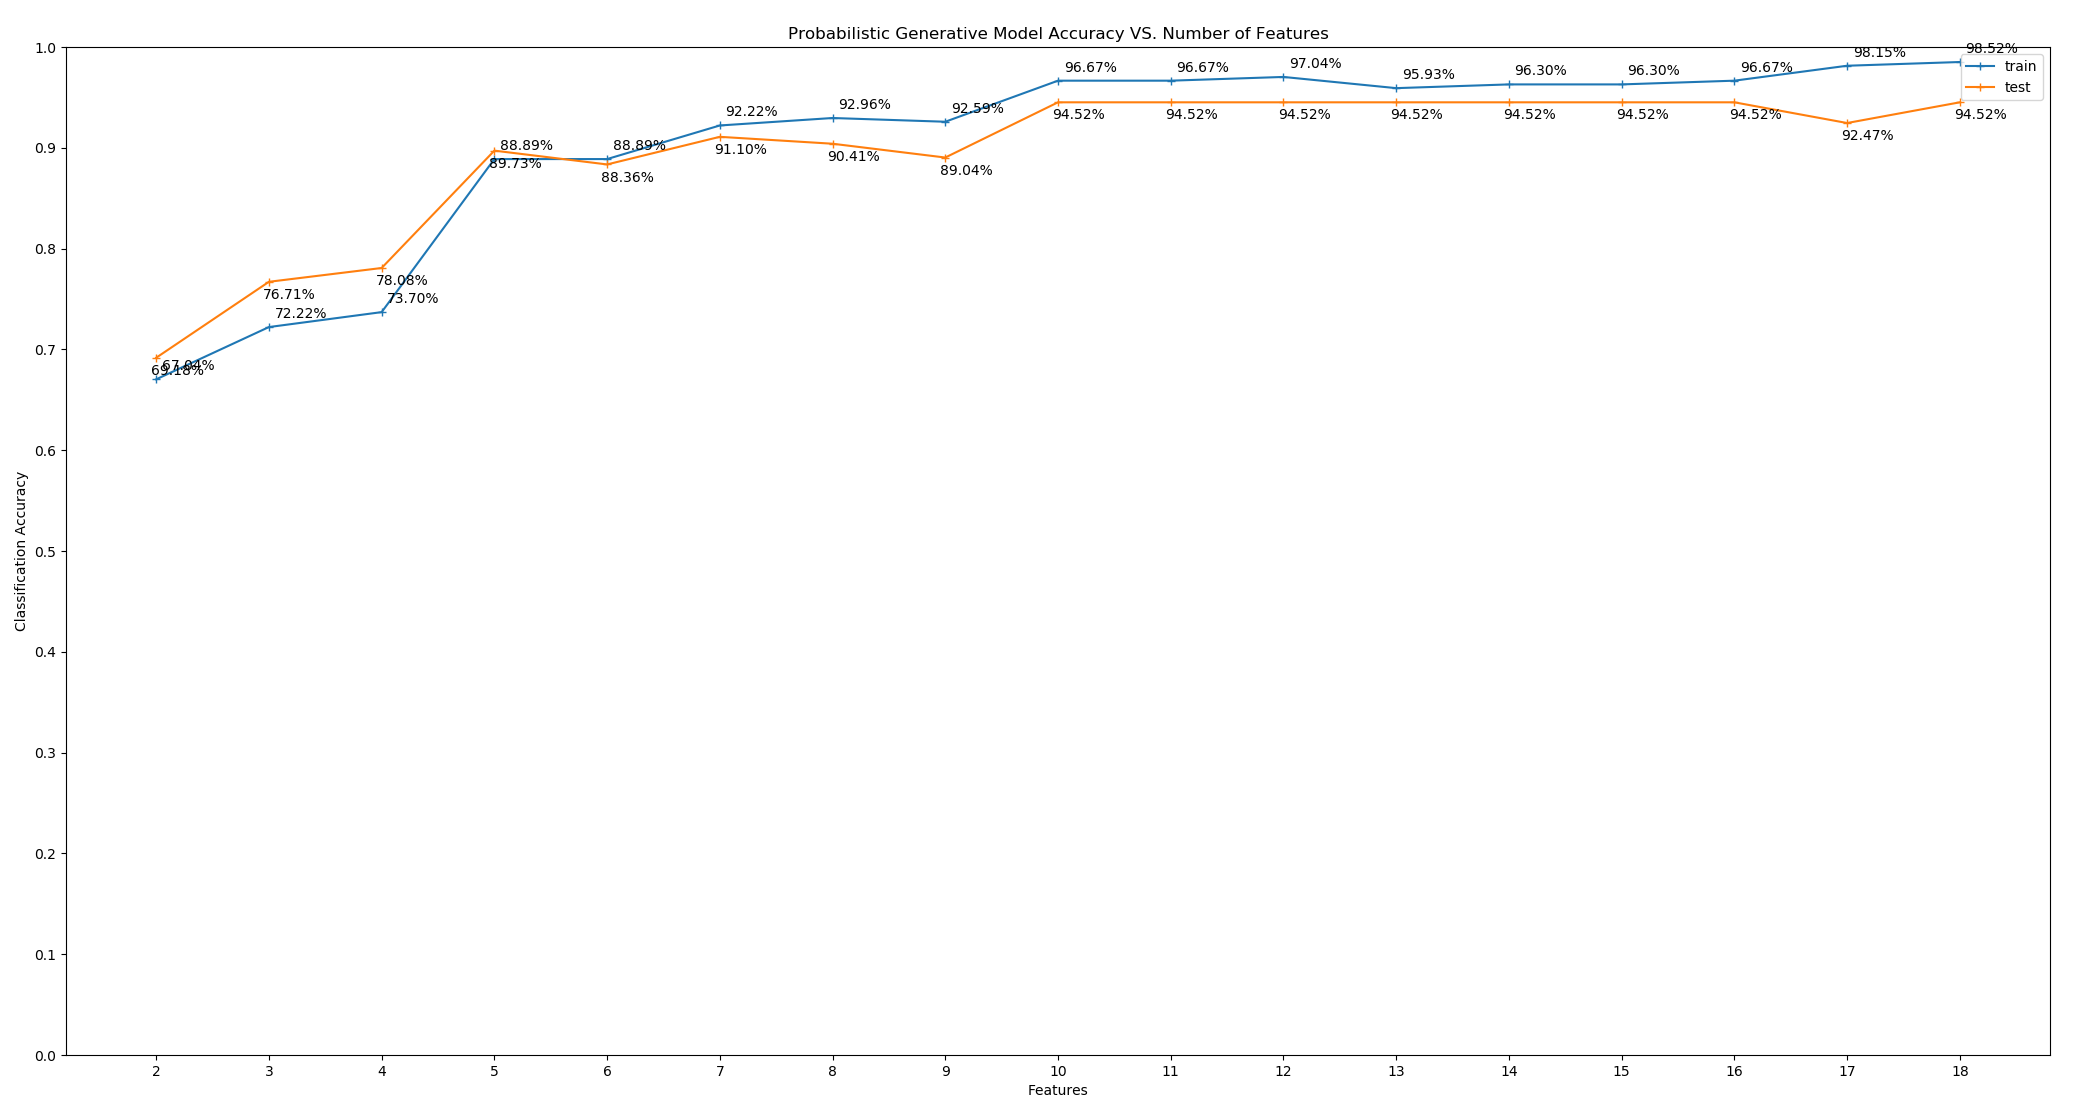
\includegraphics[scale=0.35]{pgm.png}

\subsection{Iterative Reweighted Least Squares}

We implemented the \textit{Iterative Reweighted Least Squares(IRLS)} algorithm and applied it to the dataset. 

The \textit{IRLS} update formula is:
\begin{eqnarray*}
\textbf{w}^{\textrm{new}}	&	=	&	\textbf{w}^{\textrm{old}} - H^{-1} \cdot \nabla_{\textbf{w}}E\\
	&	=	&	\textbf{w}^{\textrm{old}} - (X^TRX)^{-1} \cdot X^T(\textbf{y} - \textbf{t})\textrm{.}
\end{eqnarray*}

We initialize the weights $\textbf{w}_0$ as a column vector of Gaussian-distributed random numbers between $(-1\times10^{-4}, 1\times10^{-4})$ with $|$features$|$ elements through the code: 
\begin{lstlisting}[ language=Python,
                    deletekeywords={IDENTITY},
                    deletekeywords={[2]INT},
                    morekeywords={clustered, AUTO_INCREMENT, function, document, var, np},
                    framesep=8pt,
                    xleftmargin=40pt,
                    framexleftmargin=40pt,
                    frame=tb,
                    framerule=0pt ]
weights = np.random.uniform(low=-0.0001, high=0.0001, size=input.shape[1])[:, np.newaxis]
\end{lstlisting}
 	
We obtain $H$ by computing $X^TRX$ where $R$ is the diagonal matrix with $R_{mm} = y_m(1 - y_m)$ where $y_m = \sigma(\textbf{w}^T\textbf{x}^{(m)})$ and $\sigma(a) = \frac{1}{1 + exp(a)}$. The code is as follows:
\begin{lstlisting}[ language=Python,
                    deletekeywords={IDENTITY},
                    deletekeywords={[2]INT},
                    morekeywords={clustered, AUTO_INCREMENT, function, document, var, np},
                    framesep=8pt,
                    xleftmargin=40pt,
                    framexleftmargin=40pt,
                    frame=tb,
                    framerule=0pt ]
# numerically stable sigmoid function
sigmoid = lambda a: np.where(a >= 0, 1 / (1 + np.exp(-a)), np.exp(a) / (1 + np.exp(a)))                    

y = sigmoid(weights.reshape((1, -1)) @ input.T) # w = input
                    
def hessian(X, y):
    R = np.diag(y[0]*(1-y[0]))
    return X.T @ R @ X
\end{lstlisting}

We obtain $\nabla_\textbf{w}E$ by computing $X^T(\textbf{y} - \textbf{t}))$ where $y$ is computed as seen above, and $t$ being the normal target column vector. The code is as follows:
\begin{lstlisting}[ language=Python,
                    deletekeywords={IDENTITY},
                    deletekeywords={[2]INT},
                    morekeywords={clustered, AUTO_INCREMENT, function, document, var, np},
                    framesep=8pt,
                    xleftmargin=40pt,
                    framexleftmargin=40pt,
                    frame=tb,
                    framerule=0pt ]
def nabla_e(X, y, target):
    return X @ (y - target)
\end{lstlisting}

We obtain $\textbf{w}^{\textrm{new}}$ by updating $\textbf{w}^{\textrm{old}}$ (initially $\textbf{w}_0$ computed above) with the \textit{IRLS} update formula. We update the weights until the new \textit{negative log-likelihood error} (calculated at each iteration) differs with the previous iteration's \textit{negative log-likelihood error} by $1\times10^{-4}$ or less. Reducing the misclassification error any further is no longer efficient. The code is as follows:
\begin{lstlisting}[ language=Python,
                    deletekeywords={IDENTITY},
                    deletekeywords={[2]INT},
                    morekeywords={clustered, AUTO_INCREMENT, function, document, var, np},
                    framesep=8pt,
                    xleftmargin=40pt,
                    framexleftmargin=40pt,
                    frame=tb,
                    framerule=0pt ]
def update(weights, hessian, gradient): # IRLS update formula
    return weights - (np.linalg.inv(hessian) @ gradient)

while np.abs(error_old - error_new) > 0.0001:
        error_old = error_new

        # update until error converges
        hess = hessian(input, y)
        gradient = nabla_e(input.T, y.reshape((-1, 1)), target)
        weights = update(weights, hess, gradient)

        y = sigmoid(weights.reshape((1, -1)) @ input.T)
        error_new = log_likelihood(y.reshape((-1, 1)), target)
        [...] # out of scope code
\end{lstlisting}

The training correct classification percentage on the training set reaches a 100.00\% and 95.89\% on the test set `at' 18 features. Note that the misclassification rate is just (1.0 - \texttt{Accuracy}). The full graph can be seen below:

\hspace*{-2cm}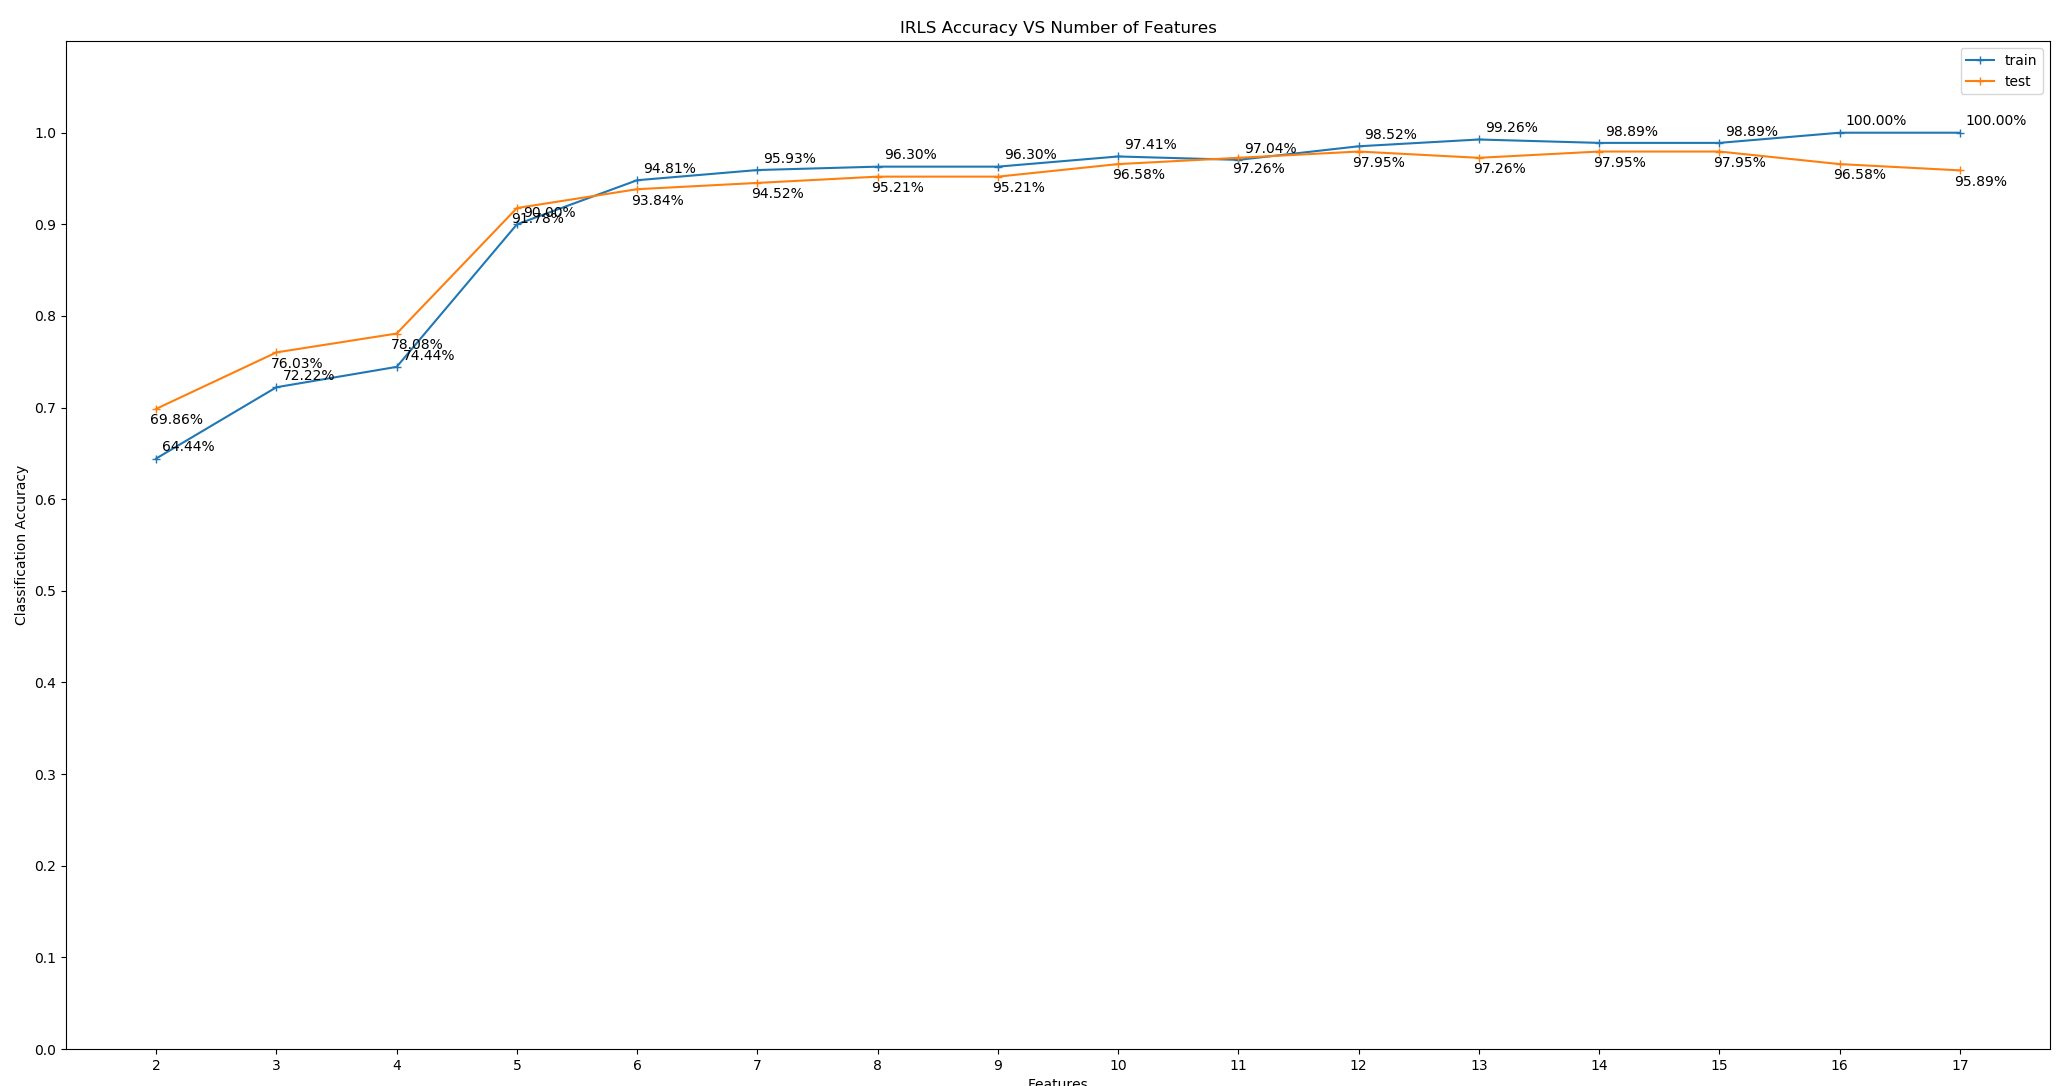
\includegraphics[scale=0.35]{irls.png}

Furthermore, we can observe the evolution of the cross-entropy error as \textit{IRLS} iterations are performed at different feature-numbers. Below we show the \textit{Cross-Entropy Error} at 3, 5, 10, and 18 features at every iteration. The last computed cross-entropies are:

\begin{tabular}{c|l}
Features	&	Negative Log-Likelihood\\\hline
3	&	[83.58347373] \\
5	&	[36.85420504] \\
10	&	[6.81522355] \\
18	&	[2.56824073e-05]
\end{tabular}

These are computed at every iteration of the \textit{IRLS} algorithm with the code:
\begin{lstlisting}[ language=Python,
                    deletekeywords={IDENTITY},
                    deletekeywords={[2]INT},
                    morekeywords={clustered, AUTO_INCREMENT, function, document, var, np},
                    framesep=8pt,
                    xleftmargin=40pt,
                    framexleftmargin=40pt,
                    frame=tb,
                    framerule=0pt ]
def log_likelihood(estimate, target):
    err_per_example = np.where(target != 0, target * np.log(estimate), 0)
    err_per_example = np.where((1-target) != 0, err_per_example + (1-target) * np.log(1 - estimate), 0)
    return -np.sum(err_per_example, axis=0)
\end{lstlisting}
\hspace*{-2cm}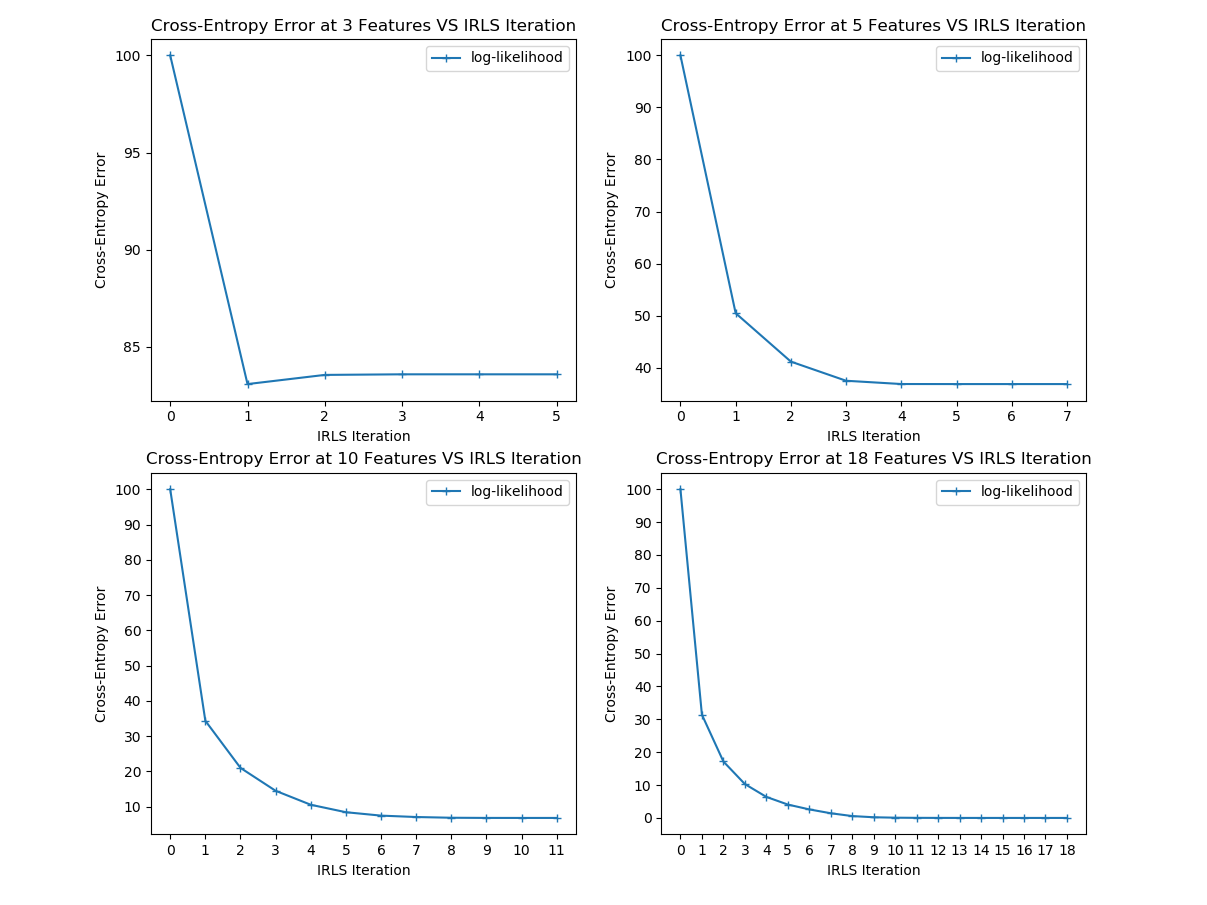
\includegraphics[scale=0.6]{irls_cee.png}

\newpage
\section{Conclusion}
We have classified the given \texttt{vehicle.pkl} dataset with the \textit{Probabilistic Generative Model} and in parallel applied the \textit{Iterative Reweighted Least Squares (IRLS)} algorithm to it. Individually, we notice the following things from each approach:
\begin{itemize}
	\item[--] \textit{Probabilistic Generative Model}: Only after including 5 features in the classification model do we get a significant jump in accuracy. However, only until the 10th feature is added do we jump to a `respectable' ($<8\%$) misclassification rate (on the test data). However, even though the accuracy on the train data increases (as expected) with the inclusion of more features, it never reaches 100\% accuracy. The misclassification rate on the test data does not decrease (strangely at 17 features it increases but is quickly corrected at the 18th feature).
	\item[--] \textit{Iterative Reweighted Least Squares (IRLS)}: Only after including 6 features in the algorithm do we get a significant jump in accuracy. Furthermore, at the 6th added feature do we jump to a `respectable' ($<8\%$) misclassification rate (on the test data). We reach 100\% accuracy on the train set at 16 added features and our lowest misclassification rate is encountered at 12, 14, and 15 added features, not after all are added, peculiarly.
\end{itemize}

When comparing both methods, we can clearly see that \textit{IRLS} is better performing than the \textit{Probabilistic Generative Model}. \textit{IRLS} reaches a `respectable' ($<8\%$) misclassification rate much earlier than the \textit{Probabilistic Generative Model}. Having less features required to reach this misclassification point makes it much more efficient - computationally cheap. At the 8th added feature, \textit{IRLS} reaches a misclassification rate the \textit{Probabilistic Generative Model} will not be able to beat. Furthermore, as more features are added from this point, \textit{IRLS} does in fact continue to improve to achieve a peak of $97.95\%$ accuracy. $3.43\%$ higher than the \textit{Probabilistic Generative Model}'s peak accuracy.


\end{document}

	\begin{lstlisting}[ language=Python,
                    deletekeywords={IDENTITY},
                    deletekeywords={[2]INT},
                    morekeywords={clustered, AUTO_INCREMENT, function, document, var, np},
                    framesep=8pt,
                    xleftmargin=40pt,
                    framexleftmargin=40pt,
                    frame=tb,
                    framerule=0pt ]

\end{lstlisting}